%==============================================================================
\chapter{Preliminaries}
\label{chapter:preliminaries}
%==============================================================================
This chapter covers the foundation technologies used throughout the thesis.
First, Section~\ref{sec:preliminaries-semantic-technologies} gives an overview about Semantic Technologies, i.e \gls{RDF} model as a standard model for representing the data and its accompanying query language \gls{SPARQL}.
It also covers different \gls{RDF} serialization formats. 
%basic concepts of the \gls{RDF} statistical criteria definition and quality assessment introduction. 
Later, Section~\ref{sec:preliminaries-distributed-frameworks} gives an introduction to \textit{Hadoop}, its core technologies \textit{\gls{HDFS}}, \textit{MapReduce} and \textit{Apache Spark} with its libraries that have been used in the course of this thesis.

\section{Semantic Technologies}
\label{sec:preliminaries-semantic-technologies}
Originally web was considered to be a hub for sharing web pages or documents that could be understood by humans.
In addition, interlinking with other web pages or records could also be generated anywhere on the web. 
Most of this data was intended solely for human consumption.
Machines could process and show such information but did not understand it.

Semantic Web~\cite{bernerslee2001semantic}, introduced by Tim Berners-Lee is an attempt to describe and link the web content into more meaningful to the machines.
The main idea is to extend the existing web considered as "Web of Documents" towards "Web of Things" a.k.a Semantic Web where things are connected and able to be exchanged with each other in an understandable way.
Semantic Web tries to give meaning to the data and thus turn the current web of documents into a more global and decentralized knowledge which is understandable and suitable for machines besides exclusively designed for human consummation.
Therefore, Semantic Web can be seen as an extension of the classical \gls{WWW}.
The Semantic Web vision is to build community-driven technologies and tools (known as standards) which allows data to be shared and reused.
As a consequence, the \gls{W3C} consortium was built and is mainly in charge of leading such standards.

\begin{figure*}
\centering
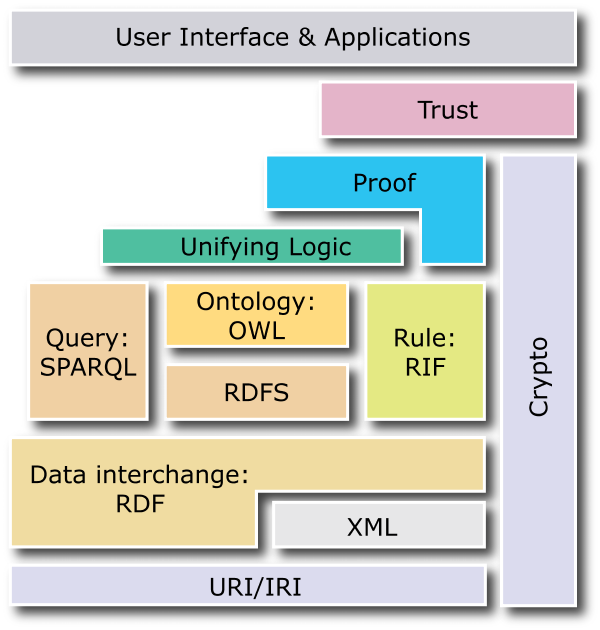
\includegraphics[width=0.7\columnwidth]{images/2_preliminaries/sw-layer-cake-2007.png}
 \caption[\textbf{Semantic Web Stack}. The Semantic Web Stack, also known as Semantic Web Cake or Semantic Web Layer Cake, illustrates the architecture of the Semantic Web, according to W3C.] %
 {\textbf{Semantic Web Stack}\footnotemark \addtocounter{footnote}{1}. The Semantic Web Stack, also known as Semantic Web Cake or Semantic Web Layer Cake, illustrates the architecture of the Semantic Web, according to W3C.}
\label{fig:preliminaries-sw-layer-cake}
\end{figure*}

Figure~\ref{fig:preliminaries-sw-layer-cake} depict various layers of Semantic Web related technologies.
Here we focus only on \textit{Data interchange: \gls{RDF}} and \textit{Query: \gls{SPARQL}} layers, which are relevant to the work presented in this thesis and are therefore discussed in this chapter.

Semantic Web's core technology is the so-called Resource Description Framework (\gls{RDF}) which serve as a main data representation.
It represent information about resources.
A resource is identified with a globally unique identifier (\gls{URI}s).
The \gls{RDF} data model can be interpreted as a directed labeled graph where resources identified by \gls{URI} are nodes in the graph and edges represent the relationships between resources labeled with the type of relationship known as predicates, also identified by \gls{URI}s.

\gls{SPARQL} is the \gls{W3C} standard for querying \gls{RDF} data.
It uses graph pattern mechanism to be matched against an \gls{RDF} graph and its syntax is similar to SQL.

More details about \gls{RDF} (cf. Section~\ref{sec:rdf-data}) and \gls{SPARQL} (cf. Section~\ref{sec:sparql}) is given in the following sections.
\addtocounter{footnote}{-1}
\footnotetext{\url{https://www.w3.org/2007/03/layerCake.png} (Retrieved in September 2019)}


\subsection{RDF Data}
\label{sec:rdf-data}

The Resource Description Framework (\gls{RDF})~\cite{Wood:14:RCA} is a \gls{W3C} standard for describing resources.
A resource is a fact or a thing which can be described and identified. 
A person, a home page, this thesis is a resource. 
An RDF resource is identified by a \emph{\gls{URI}} reference, while literals are used to represent a respective data values.
Literals consist either a string and its language tag or a value and its datatype.

An \gls{RDF} graph is a set of \gls{RDF} triples $(s,p,o)$ where $s$ is called the \emph{subject}, $p$ is the \emph{predicate} and $o$ is the \emph{object}, each of which can be an \gls{URI}, subjects and objects can alternatively be blank nodes and objects can also represent literal data values.
It can be also seen as a directed graph containing of vertices and edges. 
A vertex represent subjects and objects and an edge represent predicates.

\begin{figure*}
\centering
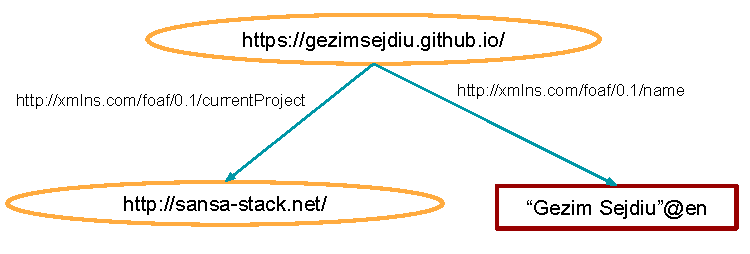
\includegraphics[width=1.0\columnwidth]{images/2_preliminaries/rdf-triple-example.pdf}
 \caption{\textbf{Sample RDF Graph representation}. Small knowledge base about 'Gezim Sejdiu' represented as a graph.}
\label{fig:preliminaries-rdf-graph-sample}
\end{figure*}
%source: https://docs.google.com/presentation/d/1a_vf-EyoC9xAcltEvTdZuT6ygoHEcC8_gayEcAhGTIY

Figure~\ref{fig:preliminaries-rdf-graph-sample} represent an \gls{RDF} graph sample about $\verb|"Gezim Sejdiu"|$ as a resource. 
One of the RDF statements (triples) from the Figure~\ref{fig:preliminaries-rdf-graph-sample} is: 

\begin{lstlisting}[basicstyle=\ttfamily,breaklines=true,showstringspaces=false,label=lst:ntriplessyntax-sample,basewidth=0.5em]
<http://sda.tech/Person/GezimSejdiu> <http://xmlns.com/foaf/0.1/currentProject> <http://sda.tech/Project/SANSAStack> .
\end{lstlisting}

which simply states "The subject identified by $\verb|<http://sda.tech/Person/GezimSejdiu>|$ has a property identified by $\verb|<http://xmlns.com/foaf/0.1/currentProject>|$ whose value is equal to $\verb|<http://sda.tech/Project/SANSAStack>|$".
In a more natural statement representation, it means that a person "Gezim Sejdiu" has a "current-project" which is "SANSA-Stack".

Below we give some necessary notions about RDF.

\begin{definition}[RDF Term]
Let $\mathcal{U}$, be a set of URIs, $\mathcal{B}$ set of blank nodes and $\mathcal{L}$ set of literals, an RDF term ($\mathcal{T}$) is a set of $\mathcal{U} \cup \mathcal{B}\cup \mathcal{L}$.
\end{definition}

\begin{definition}[RDF Triple]
Let $\mathcal{U}$, be a set of URIs, $\mathcal{B}$ set of blank nodes and $\mathcal{L}$ set of literals, an RDF triple is a ternary tuple in the form of ${(s, p, o) \in (\mathcal{U} \cup \mathcal{B}) \times \mathcal{U} \times (U \cup B \cup L)}$, where the subject $s \in (U \cup B)$ is a resource, the predicate $p \in U$ is a property, and the object $o \in (\mathcal{U} \cup \mathcal{B} \cup \mathcal{L})$ is either another resource ($\mathcal{U} \cup \mathcal{B}$) or a literal ($\mathcal{L}$).
\end{definition}

\begin{definition}[RDF Graph]
An RDF Graph ($\mathcal{G}=\{t_1, t_2, \dots , t_n\}$) is defined as a finite set of RDF triples $t_i$.
\end{definition}

\begin{definition}[RDF Dataset]
An RDF \textit{dataset} is a collection of RDF graphs $$D = \{ G_{0},\langle u_1, G_1 \rangle, \dots , \langle u_n, G_n \rangle \}$$ where $u_1, \dots , u_n \in \mathcal{U}$.
$G_0$ is considered as a default graph that does not have a name and can be empty, whereas $\langle u_i, G_i \rangle$ are called named graphs.
\end{definition}

\subsubsection{RDF Serialization Formats}
As described in Section~\ref{sec:rdf-data}, RDF is modeled as a graph where triple notation is used mostly for such representation.
In this section, we will cover some of the most common RDF serialization/syntax formats.
We focus primarily on those used during this work.

\defn{N-Triples}
The N-Triples~\cite{Seaborne:14:RN} RDF serialization format is a plain-text, line-based syntax for an RDF graph.
Each triple is written into a single line.
As a consequence, each element of the triple (\textit{subject}, \textit{predicate}, and \textit{object}) is represented without any abbreviation i.e. prefixes.
These elements then are separated with white space (spaces or tabs) and this sequence ends with a dot '$\verb|.|$' and a new line (optional at the end of a file).

\begin{lstlisting}[basicstyle=\ttfamily,breaklines=true,showstringspaces=false,label=lst:ntriplessyntax,basewidth=0.5em,caption=\textbf{N-Triples syntax example}. Representation of the example in Figure~\ref{fig:preliminaries-rdf-graph-sample} using the N-Triples syntax.,captionpos=b]
<http://sda.tech/Person/GezimSejdiu> <http://www.w3.org/1999/02/22-rdf-syntax-ns#type> <http://xmlns.com/foaf/0.1/Person> .
<http://sda.tech/Person/GezimSejdiu> <http://xmlns.com/foaf/0.1/name> "Gezim Sejdiu"@en .
<http://sda.tech/Person/GezimSejdiu> <http://xmlns.com/foaf/0.1/homepage> <https://gezimsejdiu.github.io/> .
<http://sda.tech/Person/GezimSejdiu> <http://xmlns.com/foaf/0.1/currentProject> <http://sda.tech/Project/SANSAStack> .
<http://sda.tech/Project/SANSAStack> <http://www.w3.org/1999/02/22-rdf-syntax-ns#type> <http://xmlns.com/foaf/0.1/Project> .
<http://sda.tech/Project/SANSAStack> <http://www.w3.org/2000/01/rdf-schema#label> "Semantic Analytics Stack (SANSA)"@en .
<http://sda.tech/Project/SANSAStack> <http://xmlns.com/foaf/0.1/homepage> <http://sansa-stack.net> .
\end{lstlisting}

Listing~\ref{lst:ntriplessyntax} is an N-Triples representation of the example depicted in Figure~\ref{fig:preliminaries-rdf-graph-sample}.

As we see from the N-Triples basic example above, $\verb|URI|$s are written between angle brackets i.e. '$\verb|<|$' and '$\verb|>|$'.
Literals are enclosed by double quotes. 
Sometimes, literals include language tags using a '$\verb|@|$' symbol and if typed, with '$\verb|^^|$'.
Blank nodes are identified by '$\verb|_:|$'.

\defn{Turtle}
The Turtle~\cite{Carothers:14:RT} syntax is basically a textual syntax for an RDF.
It is a more compact and natural form to write an RDF graph as compared i.e. N-Triples syntax.
Turtle can bee seen as an extension of the N-Triples representation, with abbreviations for common usage patterns and datatypes.
Triples written in Turtle are a sequence of \textit{subject}, \textit{predicate} and \textit{object} separated by a white space (spaces or tabs) this sequence ends with a dot '$\verb|.|$' like in N-Triples.

With the Turtle syntax, RDF statements can be written in a more compact way as compared to N-Triples.
Often, triples are grouped (1) if several \textit{predicates} share the common \textit{subject}, and (2) if the same tuple (\textit{subject}, \textit{predicate}) have multiple object values. 
The following example depict an RDF graph represented in a Turtle syntax.

\begin{lstlisting}[basicstyle=\ttfamily,breaklines=true,showstringspaces=false,label=lst:turtlesyntax,basewidth=0.5em,caption=\textbf{Turtle syntax example}. Representation of the example in Figure~\ref{fig:preliminaries-rdf-graph-sample} using the Turtle syntax.,captionpos=b]
@base               <http://sda.tech/> .
@prefix rdf:        <http://www.w3.org/1999/02/22-rdf-syntax-ns#> .
@prefix rdfs:       <http://www.w3.org/2000/01/rdf-schema#> .
@prefix foaf:       <http://xmlns.com/foaf/0.1/> .
@prefix sdaperson:  <http://sda.tech/Person/> .
@prefix sdaproject: <http://sda.tech/Project/> .

sdaperson:GezimSejdiu a foaf:Person ;
                   foaf:name "Gezim Sejdiu"@en ;
                   foaf:homepage <https://gezimsejdiu.github.io/> ;
                   foaf:currentProject sdaproject:SANSAStack .

sdaproject:SANSAStack a foaf:Project ;
                 rdfs:label "Semantic Analytics Stack (SANSA)"@en ;
                 foaf:homepage <http://sansa-stack.net> .
\end{lstlisting}

Listing~\ref{lst:turtlesyntax} represent the example depicted in Figure~\ref{fig:preliminaries-rdf-graph-sample} in the Turtle syntax.
This example introduces some of the features of the Turtle language: prefixes defined by the '$\verb|@|$' symbol, predicated lists separated by '$\verb|;|$', and literals.
The object lists are separated by '$\verb|,|$' in case they share the same tuple (\textit{subject}, \textit{predicate}).

\defn{RDF/XML}
The RDF/XML~\cite{Schreiber:14:RXS} is an XML representation of an RDF graph.
It is considered a normative syntax and the RDF graph is encoded using XML terms -- element names, attribute names, element contents and attribute values.
It exploit a hierarchical structure for representation of an RDF graph.
An RDF graph using the RDF/XML representation is considered as a collection of paths (in the hierarchical structure) of the form $node \longrightarrow predicate~arc \longrightarrow node \longrightarrow predicate~arc \longrightarrow node \longrightarrow predicate~arc, \dots \longrightarrow node$ which cover the entire graph.
These paths then become a sequence of elements within elements that alternate node elements with arcs predicates.

\begin{lstlisting}[basicstyle=\ttfamily,breaklines=true,showstringspaces=false,label=lst:rdfxmlsyntax,basewidth=0.5em,caption=\textbf{RDF/XML syntax example}. Representation of the example in Figure~\ref{fig:preliminaries-rdf-graph-sample} using the RDF/XML syntax.,captionpos=b]
<?xml version="1.0" encoding="UTF-8"?>
<rdf:RDF
	xmlns:rdf="http://www.w3.org/1999/02/22-rdf-syntax-ns#"
	xmlns:rdfs="http://www.w3.org/2000/01/rdf-schema#"
	xmlns:foaf="http://xmlns.com/foaf/0.1/"
	xmlns:sdaperson="http://sda.tech/Person/"
	xmlns:sdaproject="http://sda.tech/Project/">

<rdf:Description rdf:about="http://sda.tech/Person/GezimSejdiu">
	<rdf:type rdf:resource="http://xmlns.com/foaf/0.1/Person"/>
	<foaf:name xml:lang="en">Gezim Sejdiu</foaf:name>
	<foaf:homepage rdf:resource="https://gezimsejdiu.github.io/"/>
	<foaf:currentProject rdf:resource="http://sda.tech/Project/SANSAStack"/>
</rdf:Description>

<rdf:Description rdf:about="http://sda.tech/Project/SANSAStack">
	<rdf:type rdf:resource="http://xmlns.com/foaf/0.1/Project"/>
	<rdfs:label xml:lang="en">Semantic Analytics Stack (SANSA)</rdfs:label>
	<foaf:homepage rdf:resource="http://sansa-stack.net"/>
</rdf:Description>

</rdf:RDF>
\end{lstlisting}

Listing~\ref{lst:rdfxmlsyntax} represent an RDF/XML syntax of the example in Figure~\ref{fig:preliminaries-rdf-graph-sample}. 
The $\verb|rdf:RDF|$ node is consider as a root node of an RDF/XML document.
RDF triples are grouped according to their subject and encoded using the XML elements.
The $\verb|rdf:Description|$ is the node element and is used to describe subjects and objects of the RDF graph.
The $\verb|rdf:about|$ attribute is used for the unique identifier of a resource representation, whereas the literal values are encoded using the separate tags (e.g. $\verb|rdfs:label|$, $\verb|foaf:name|$).
The property elements (predicates) can either be encoded using the XML attributes or as a separate resources i.e using the $\verb|rdf:resource|$ element.

\subsection{SPARQL}
\label{sec:sparql}
An \gls{RDF} graph is considered being a directed, labeled graph data format which represent information in the Web.
\gls{SPARQL}~\cite{Seaborne:08:SQL} is a \gls{W3C} standard query language for retrieving and manipulating RDF data.
Its core component is the graph pattern mechanism which allows users to write queries in the form of triple patterns, conjunctions, disjunctions and/or a set of optional patterns (e.g. $\verb|FILTER|$) which are matched against an RDF graph.
This is done by replacing the variables in the triple pattern with elements fo the RDF graph such that the resulting graph is contained in the original RDF graph, known as pattern matching.
The results of SPARQL queries are set of binding or an RDF graph.

In the following we cover the foundation of SPARQL and its syntax as an analogue to the definitions in~\cite{Perez:2009:SCS:1567274.1567278}.
More details can also be found in the W3C specification of SPARQL~\cite{Seaborne:08:SQL}.


\begin{definition}[Triple Pattern]
Let $\mathcal{V}$ be a set of variables such that $ \mathcal{V} \cap \mathcal{T} = \emptyset $. 
A triple pattern $tp$ is member of the set ($\mathcal{T} \cup \mathcal{V}) \times (\mathcal{U} \cap \mathcal{V}) \times (\mathcal{T} \cup \mathcal{V})$.
\end{definition}

\begin{definition}[Query Variable]
A query variable is a member of the set $\mathcal{V}$ where $\mathcal{V}$ is considered infinite and disjoint from $\mathcal{T}$ .
\end{definition}

\begin{definition}[Basic Graph Pattern (BGP)]
Let $tp = \{ tp_1, tp_2, tp_3, \dots , tp_n \}$ be a set of triple patterns. 
A Basic Graph Pattern $BGP$ is a conjunction of triple patterns, i.e  $BGP = tp_1 \wedge tp_2 \wedge tp_3 \wedge , \dots , \wedge tp_n$.
\end{definition}

\begin{definition}[Solution Modifiers]
A solution modifiers is a mapping from a set of $\mathcal{V}$ to a set of $\mathcal{T}$.
More formally, $SM= \{ (v, modifier(v))| v \in \mathcal{V}$, where $modifer$ is one of the \verb|project|, \verb|distinct|, \verb|order|, \verb|limit|, and \verb|offset| modifiers.
\end{definition}

\begin{definition}[Result Set]
Given $Q = (BGP, D, SM, SELECT~\mathcal{V})$, then a result set $QS$ is a solution formed by matching dataset $D$ with graph pattern $BGP$. 
\end{definition}

\begin{definition}[SPARQL Query]
A SPARQL query is a tuple $(BGP, D, SM, QS)$.
\end{definition}

Let us consider an example for better understanding of SPARQL.
Assume that we want to know "\textit{What is the project (and its homepage) that Gezim Sejdiu is currently working on?}" from our small knowledge base (as depicted in Figure~\ref{fig:preliminaries-rdf-graph-sample}).
Listing~\ref{lst:sparqlexample} depict a simple SPARQL query to retrieve information about the project and its homepage of Gezim Sejdiu's current project.


\begin{lstlisting}[basicstyle=\ttfamily,breaklines=true,showstringspaces=false,morekeywords={PREFIX,SELECT,WHERE,OPTIONAL,FILTER,java,rdf,rdfs,url},numbers=left,stepnumber=1,label=lst:sparqlexample,basewidth=0.5em,caption=\textbf{A SPARQL query example}. A SPARQL query to retrieve the project name and its homepage of Gezim Sejdiu's current project (as depicted in Figure~\ref{fig:preliminaries-rdf-graph-sample}).,captionpos=b,xleftmargin=1.5em]
PREFIX sda:       <http://sda.tech/>
PREFIX sdaperson: <http://sda.tech/Person/>
PREFIX foaf:      <http://xmlns.com/foaf/0.1/>

SELECT ?project ?homepage
WHERE {
     sdaperson:GezimSejdiu foaf:currentProject ?project.
     ?project foaf:homepage ?homepage. 
}
\end{lstlisting}

We see that (from Listing~\ref{lst:sparqlexample}) SPARQL query has a similar SQL-like syntax.
Mainly a SPARQL query contains four parts. 
First, prefixes as optional header are given. 
It help the reader to make the rest of the query more readable.
Second, the query form is defined. 
In our case we use $\verb|SELECT|$ query form.
Then, the $\verb|WHERE|$ clause is used which is the main definition of the SPARQL query.
It involves a set of conditions/patterns as a composition of the result set.
Finally, optional solution modifiers are set in order to adjust the selection before retrieving the results.

More specifically, in Listing~\ref{lst:sparqlexample}, lines 1-3 define prefixes as a shortness version of \gls{URI}s.
The upcoming statement (line 5) is the $\verb|SELECT|$ clause which declares the variables that should be retrieved as an output when executing the query.
There are two variables $\verb|?project|$ and $\verb|?homepage|$.
We see that variables are defined with a $\verb|?|$ symbol.
The following statements (lines 7-8) include two BGPs.
The first one (line 7) states that the statement with subject $\verb|sdaperson:GezimSejdiu|$ and property $\verb|foaf:currentProject|$, we assign the value of its object to a variable called $\verb|?project|$.
When evaluated, this variable will contain the value of $\verb|sdaproject:SANSAStack|$.
Afterwords (line 8), the same variable $\verb|?project|$ with an associated value will be the subject of the next statement.
That is, the statement will be $\verb|sdaproject:SANSAStack foaf:homepage ?homepage|$.
The remaining variable $\verb|?homepage|$ then will take the value $\verb|http://sansa-stack.net|$.
As an output, both values of the variables $\verb|?project|$ and $\verb|?homepage|$ will be rendered.

\section{Hadoop Ecosystem}
\label{sec:preliminaries-distributed-frameworks}
Apache Hadoop~\cite{White:2015:HDG:2904397} is a collection of distributed processing and storage frameworks of large-scale datasets across a cluster of computers.
Its ecosystem contains a build-in mechanisms in order to guarantee fault tolerance and high availability on top of commodity hardware.
Therefore, specific hardware involvement is not needed, making it highly scalable and cost-effective.

As of today, Hadoop ecosystem has been enriched with an extensive tools and libraries that are either built on top of Hadoop or use it for different application fields, including but not limited to: data mining, querying, data analysis, processing and data warehousing.
It has become the de-facto industry standard in the Big Data management all thanks to its high degree of parallelism, fault-tolerant, reliability and scalability.

In this section, we provide a brief overview of the Hadoop ecosystem projects used in the course of this thesis.
We focus mostly on the aspects needed to understand the content of the following chapters without going into the technical details.

\subsection{Apache Hadoop and MapReduce}

\subsubsection{HDFS}
\label{sec:hdfs}
The Hadoop Distributed File System (\gls{HDFS})~\cite{Shvachko:2010:HDF:1913798.1914427} is one of the main components of the Hadoop. 
It is a popular file system capable of handling the distribution of the data across multiple nodes in the cluster.
\gls{HDFS} serve as a common, distributed and fault-tolerant data pool for all applications on top of the Hadoop in order to minimize the data movement and duplication.
Furthermore, it also leverage the distributed processing of large-scale datasets by adapting advanced and automatically partitioning techniques across all the nodes in the cluster.
\gls{HDFS} was originally built as infrastructure for the Apache Nutch\furl{https://nutch.apache.org/} web search engine project and was inspired by the \gls{GFS}~\cite{Ghemawat:2003:GFS:945445.945450}. 
\gls{HDFS} is an integral component of the Apache Hadoop ecosystem.

\gls{HDFS} is designed in a way that it doesn't require highly reliable and costly hardware but instead, it can be run on a cluster of computers with commodity hardware.
HDFS splits data (files) into blocks that can be replicated across the cluster in order to ensure fault-tolerance and efficiency.

The \gls{HDFS} architecture follows the master/slave model. 
The \textit{namenode} (master) is responsible for managing a file system namespace or a directory structure, coordinating replication process, keep track and maintain metadata about the replicated blocks.
The \textit{datanodes} (slaves) are the machines where these blocks are physically stored.
A \textit{datanode} instance allows access for storing and retrieving the data. 
To increase the availability, the \textit{namenode} maintains multiple copies of the metadata of the replicated blocks.
In the earlier version of \gls{HDFS}, the \textit{namenode} was consider being a single point of failure.
Latest versions support deploying two instances configured being \textit{namenode} with the mechanism active/passive for a high availability.
An active \textit{namenode} is the \textit{namenode} which is running in the cluster, and a passive \textit{namenode} is kept synchronized and stand by.
In case of a failure, the passive \textit{namenode} can replace the active \textit{namenode}.
Hence, the cluster can be recovered faster and it never fails.

\subsubsection{MapReduce}
Beside its distributed file system, Hadoop contains computing system so-called MapReduce~\cite{dg2004mapreduce}.
MapReduce is a distributed framework that allows for the distributed processing of large data sets across a cluster of computers.
It enables scalable, fault tolerant and massively parallel computations over a cluster of machines.
The core of MapReduce is a distributed file system \gls{GFS} which split larger size of files into equal sized blocks of records across the cluster. 

\begin{figure*}
\centering
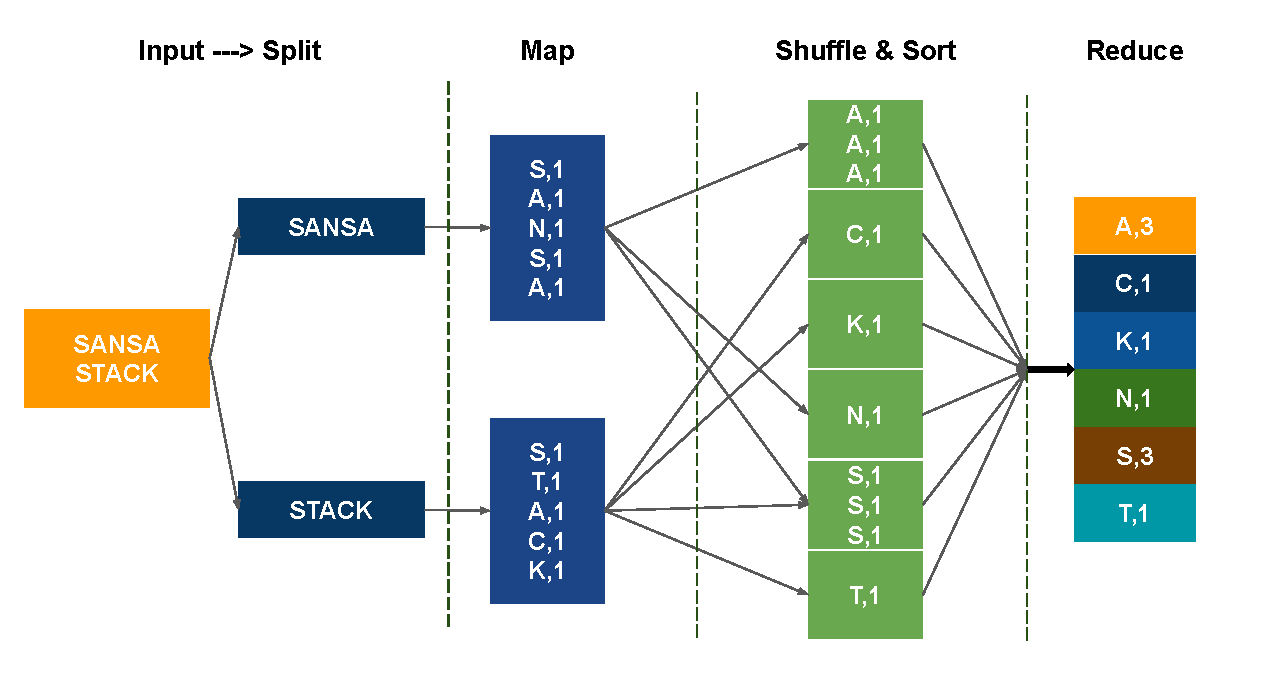
\includegraphics[width=1.0\columnwidth]{images/2_preliminaries/mapreduce-dataflow.pdf}
 \caption{\textbf{MapReduce dataflow}. A MapReduce dataflow illustrated with "Character Count" example.}
\label{fig:preliminaries-mapreduce-dataflow}
\end{figure*}
%source: https://docs.google.com/presentation/d/1SlluoX2aceY2uRguuqxXfLB7yJIqsR_dBK8AUgTvPjE


The workflow of a MapReduce job is a sequence of \textit{map} and \textit{reduce} phases performed in an iterative way.
These phases contains a \textit{shuffle} and \textit{sort} operations (as depicted in Figure~\ref{fig:preliminaries-mapreduce-dataflow}) as an intermediate phase.
Usually, the input data is split into a distributed blocks across the cluster for parallel execution.
Topically, a program should contain the \textit{map} and \textit{reduce} operations which are then evaluated in a parallel setting on a partition of the data.
During the \textit{map} phase, every record of the input dataset as key/value pairs is read and another set of intermediate key/value pairs is generated.
Later, during the \textit{reduce} phase these key/value pairs are ingested and evaluated in order to return a single set of results.
While performing such map/reduce phases, intermediate results are generated and need to be shuffled and/or sorted across the cluster.

The  user has to implement the \textit{map} and \textit{reduce} functions with a signature as follows:

\begin{verbatim}
    map:    <k1, v1> --> Map() --> list(<k2, v2>)
    reduce: <k2, list(v2)> --> Reduce() --> list(<k3, v3>)
\end{verbatim}

Figure~\ref{fig:preliminaries-mapreduce-dataflow} illustrates an example of the MapReduce dataflow.
With such example, user wants to count the number of occurrences for all characters in the dataset.
First, the input is split into a small subsets of the dataset, e.g. a line of text.
The map function splits the input into a set of characters and output the key/value pairs, i.e. \textit{(character, 1)} for every character occurrence.
Later, the shuffle \& sort phase is used to combine and partition all the pairs with the same key (character) to the same reducer and thus the reduce function is executed with a list of values for a single character.
Finally, the sum of all these values is returned.

\subsection{Apache Spark}
Apache Spark\furl{http://spark.apache.org/} is a fast and generic-purpose cluster computing engine which is built over the Hadoop ecosystem.
It started as a research project in 2009 within the AMPLab\furl{https://amplab.cs.berkeley.edu/} at the Unviersity of California, Berkeley.
The main goal of the project was to keep the benefits of the MapReduce's scalable, distributed, and fault-tolerant processing framework while making it more efficient and much easier to use.

Apache Spark follows a master/slave architecture, i.e. one central coordinator and many distributed workers.
A Spark cluster contains a single master, a cluster manager and any number of workers (slaves).
Figure~\ref{fig:preliminaries-spark-dataflow} depict a cluster mode overview architecture of Spark.
Spark applications can run as an independent sets of processes on the cluster, coordinated by the so-called \textit{SparkSession} in the \textit{driver program}.
More specifically, a Spark session connects to a cluster manager (e.g. Spark's own standalone cluster manager), which allocate resources across applications when run on the cluster.
Once connected to the cluster manager, it acquires executors on the worker nodes, which are processes that run computations and store data for the submitted application.
Afterword, it sends the application code to the executors. 
Hence, the tasks are triggered to run on those executors, one task per partition.
Such a task applies its workload to a dataset in its partition and outputs a new partition dataset.
Some of the tasks performed on Spark may involve iterative operations where operations are run repeatedly to data, they benefit from caching datasets across iterations.
Finally, the results are sent back to the driver application.
They can be kept in-memory for further processing or pushed back and saved to disk.

\begin{figure*}
\centering
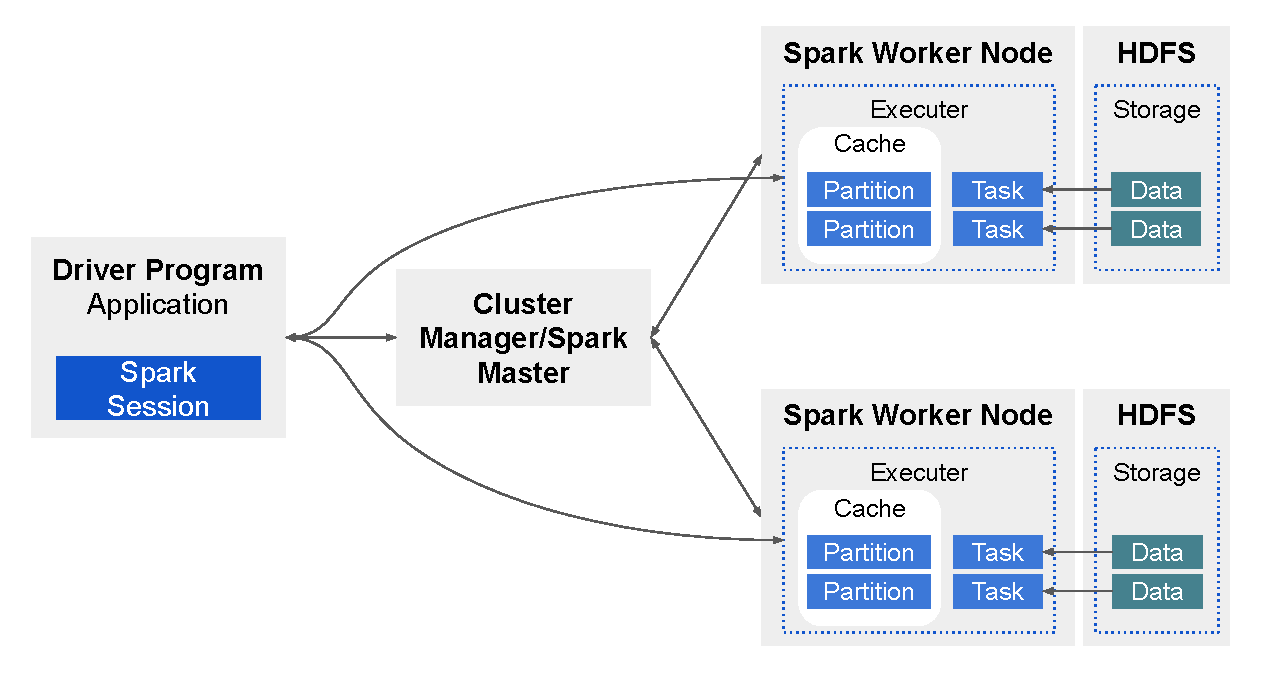
\includegraphics[width=1.0\columnwidth]{images/2_preliminaries/spark-dataflow.pdf}
 \caption{\textbf{Spark Architecture Diagram}. A Spark Cluster Mode Overview.}
\label{fig:preliminaries-spark-dataflow}
\end{figure*}
%source: https://docs.google.com/presentation/d/15hAaL75__sxYyxAZDM8ysZuu8aVxntCqHucZ1-fFLX4

The main data structures that Spark operates with are so-called \gls{RDD}~\cite{zaharia2012resilient} which are a fault-tolerant and immutable collections of records that can be operated in a parallel setting.
\gls{RDD}s are considered being \textit{resilient} -- fault-tolerant and capable of rebuilding data on failure, \textit{distributed} -- able to distribute the data among the multiple nodes in the cluster, and \textit{dataset} -- collection of partitioned data with their values.
An \gls{RDD} splits the data into chunks based on a key. 
They are considered being highly resilient i.e being able to recover quickly from any failure as the same data chunks are replicated across multiple executor nodes in the cluster.
Thus, even a node failure occur, the other nodes will still process the data.
Moreover, an \gls{RDD}, once created becomes immutable -- not able to be modified after it is created.
\gls{RDD} follow the concept of transformation and are considered being lazy evaluation.

In a distributed setting, each dataset in \gls{RDD} is split into logical partitions which are computed on different nodes in the cluster.
This allows us to perform any transformation or action on the whole dataset in a parallel manner.
The distribution of the workload is taken care by Spark.
Such an \gls{RDD} can be created using an existing collection of the data or by loading a dataset from an external storage system, such as \gls{HDFS}, or even a file system.
With \gls{RDD}s, we can perform two types of operations: (i) \textit{Transformations} -- operations which are applied when creating an \gls{RDD} or transforming it to another one, and (ii) \textit{Actions} -- operations applied on an \gls{RDD} and retrieve the result.

Apache Spark provides a rich set of APIs for faster, in-memory processing of \gls{RDD}s.
It also provides a rich functional programming model and comes with higher level libraries, e.g. for structured querying (\textit{Spark SQL}), machine learning (\textit{MLlib}), streaming (\textit{Spark Streaming}), and graph parallel processing (\textit{GraphX}).

In the following sections, we will cover those libraries we make use of.

\subsubsection{GraphX}
GraphX~\cite{Gonzalez2014GraphX} is a Spark library for graphs and parallel graph computation.
It extends the \gls{RDD} abstraction and thus introduces \gls{RDG}, which relates records with vertices (VertexRDD) and edges (EdgeRDD) in a graph and provides an expressive set of computational primitives.
In addition, GraphX simplifies the conventional ETL processes and analysis significantly by providing new operations for viewing, filtering, and transforming graphs.

The GraphX \gls{RDG} leverages advances in distribtued graph representation by comining best of both worlds; benefits of graph-parallel and data-parallel systems.
It exploits the graph structure in order to minimize the network communication and storage overhead.

It uses the so-called efficient vertex-cut partitioning strategy (as described in~\cite{Gonzalez2012PowerGraph}) and data-parallel partitioning heuristics by assigning edges to machines and allowing vertices to span multiple machines in order to minimize the vertex span per machine.
By adding an abstraction to the core of Spark (\gls{RDD}s) it ease the usage of graph data.
GraphX contains a set of common graph operations, i.e \textit{filter}, \textit{map}, \textit{reduceByKey}, \textit{join}, etc.
By using such graph-parallel and data-parallel operations, GraphX perform its computation.
Usually, these operators take a graphs and collections as an input and produce new graphs and collections as an output.


\subsubsection{SparkSQL}
Spark SQL~\cite{Armbrust2015SSR} is a Spark library for SQL and structured data processing which allows querying structured data inside Spark programs.
Essentially, the main abstraction in Spark SQL’s API is a \textit{DataFrame} which are a distributed collections of rows with a homogeneous schema.
A \textit{DataFrame} is an \gls{RDD} with a schema.
They can be seen as tables in a relational database and can also be manipulated in a similar ways to \gls{RDD}s.
They are represented using a columnar storage format (while kept in-memory caching) which allows access to only those columns required, therefore it reduces the memory footprint by applying a columnar compression schemas, i.e dictionary encoding and run-length encoding.
The main purpose of using DataFrames as compared to \gls{RDD}s is that it offer a built-in optimizer for Spark SQL operators, the \textit{Catalyst}.
It leverages advanced programming language features (e.g. Scala’s pattern matching) in order to build an extensible query optimizer by scanning the data schema and its query semantics.

Spark DataFrames are considered being lazy, as a consequence, each DataFrame object represents a logical plan to compute a dataset, but no real execution occurs until an action is called, i.e. count.
By this, Spark enables rich optimization across all operations which has been used in order to build a DataFrame.


